\section{Effect Of Aging On $\dfrac{\Delta{u}}{p}-\varepsilon$ Relationship 时效对$\dfrac{\Delta{u}}{p}-\varepsilon$关系的影响}

\begin{paracol}{2}
    
    The change of pore-pressure ratio $\Delta{u}/p$ in relation to strain for all the samples consolidated isotropically and anisotropically are plotted in \autoref{figure:4a} and \autoref{figure:4b}, respectively.

    \switchcolumn

    对于各向同性和各向异性固结的所有样品,孔隙压力比$\Delta{u}/p$随应变的变化分别绘制在\cnsubfigureref{figure:4a}和\cnsubfigureref{figure:4b}中。

    \switchcolumn*

    \autoref{figure:4a} shows clearly that in spite of the different period of aging a unique relationship exists between excess pore-pressure and major principal strain. The points resulting from the performed six tests on the isotropically consolidated samples fall very close to a single curve. The conclusion may therefore be reached that aging has no effect on the porepressure/strain relationship.

    \switchcolumn
        
    \cnsubfigureref{figure:4a}清楚地表明,尽管老化时间不同,但在超孔隙压力和主要主应变之间仍存在独特的关系。 对各向同性固结样品进行六次试验所得的点非常接近一条曲线。 因此可以得出结论,时效对孔压/应变关系没有影响。

    \switchcolumn*

    \autoref{figure:4b} are plotted the excess pore pressures observed during the shearing of the anisotropically consolidated samples. These test results show a considerable scatter, but a detailed study shows that the variation of the observed pore pressures does not correspond to or is not correlated with any specific variable such as time of aging or the water content. It is believed, therefore, that the scatter is a result of small variations of principal stress ratio during the consolidation \citep{Lo1961219}.

    \switchcolumn
        
    在\cnsubfigureref{figure:4b}中,绘制了在各向异性固结样品剪切过程中观察到的多余孔隙压力。 这些试验结果显示出相当大的分散性,但是详细的研究表明,观察到的孔隙压力的变化与任何特定变量(例如老化时间或含水量)不对应或不相关。 因此,可以认为,分散是固结过程中主应力比的微小变化的结果\citep{Lo1961219}。

\end{paracol}

\begin{figure}[!htbp]
    \centering
    \subfigure[CIU, tests on isotropically consolidated samples]{
        \label{figure:4a}
        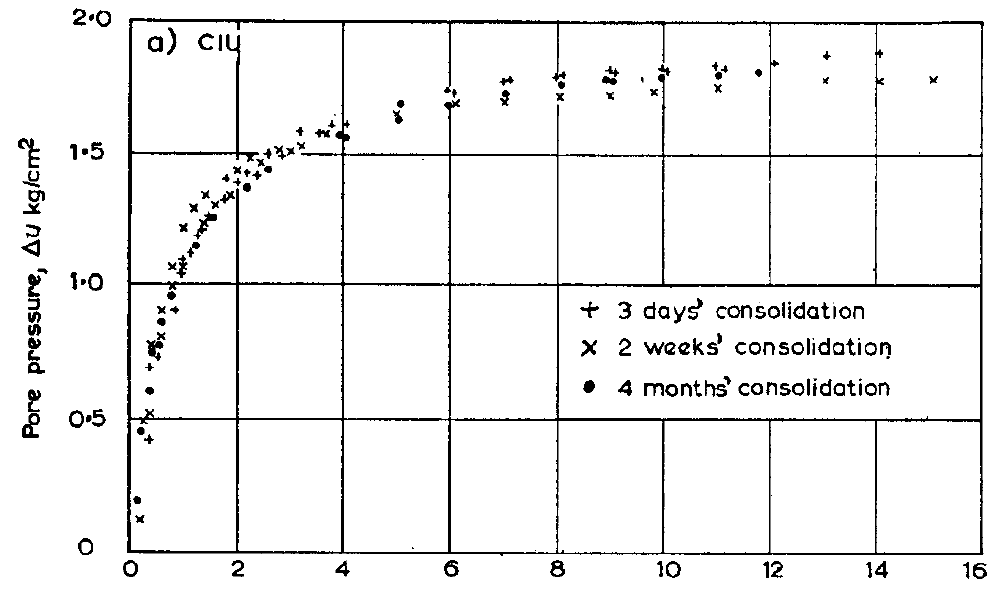
\includegraphics[width=0.43\textwidth]{figures/figure-4a.png}
    }
    \subfigure[CAU, tests on anisotropically consolidated samples]{
        \label{figure:4b}
        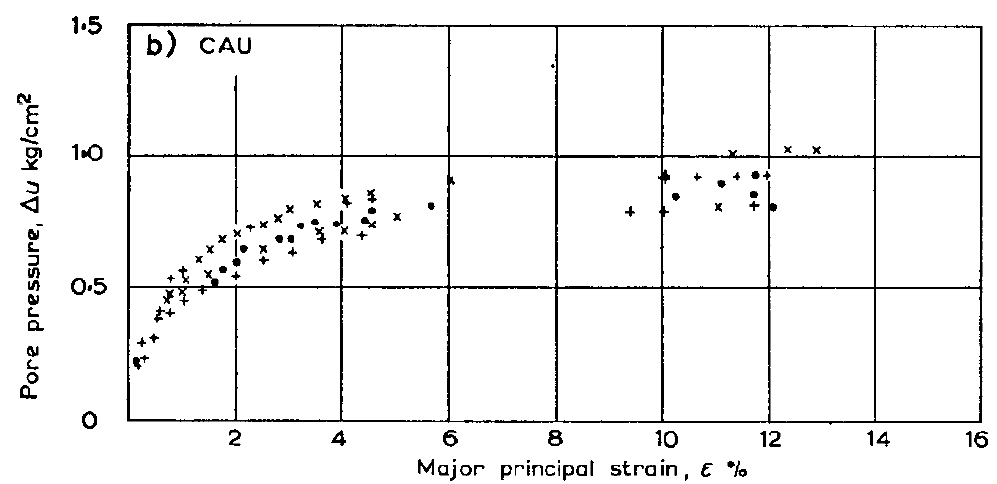
\includegraphics[width=0.53\textwidth]{figures/figure-4b.png}
    }
    \caption{Excess pore pressure set up during consolidated undrained tests, For each type of consolidation are shown the results of six separate tests.}
    \addtocounter{figure}{-1}
    \vspace{-5pt}
    \renewcommand{\figurename}{图}
    \caption{在固结不排水的综合试验中设置了过多的孔隙压力,对于每种类型的固结试验,均显示六个独立试验的结果。}
    \renewcommand{\figurename}{Figure}
    \label{figure:4}
\end{figure}

\begin{paracol}{2}
    

    The maximum values of $\Delta{u}/p+(1-K)$ are listed in \autoref{table:3} for comparison. The values determined for the anisotropically consolidated samples are slightly higher than those observed for the isotropical samples, a finding which has been confirmed also for other types of clay \citep{Bjerrum196123b}. The tests on the isotropical samples show no tendency for this quantity to vary with the time of aging, but a small increase with time of aging was observed for the samples consolidated anisotropically.

    \switchcolumn

    \cntableref{table:3}中列出了$\Delta{u}/p+(1-K)$的最大值以进行比较。 各向异性固结样品的测定值略高于各向同性样品的观察值,这一发现在其他类型的黏土中也得到了证实\citep{Bjerrum196123b}。在各向同性样品上进行的试验表明,该数量没有随老化时间变化的趋势,但对于各向异性固结的样品,随老化时间的增加却很小。

\end{paracol}